%% Los capitulos inician con \chapter{T'itulo}, estos aparecen numerados y
%% se incluyen en el 'indice general.
%%
%% Recuerda que aqu'i ya puedes escribir acentos como: 'a, 'e, 'i, etc.
%% La letra n con tilde es: 'n.

\chapter{Pruebas y Resultados}

En este capitulo se explican en detalle los resultados y pruebas realizadas para garantizar que el funcionamiento y rendimiento de cada módulo cumpla los objetivos establecidos para el sistema.

\section{Pruebas de Módulos}

A continuación se presentan las pruebas realizadas por cada módulo del sistema.

\subsection{Modelo}

Para validar el modelo se realizaron varias pruebas y análisis de la información obtenida, estas fueron las conclusiones obtenidas.

\subsubsection{Matriz de Frecuencia, Recencia y Compras Esperadas}

Inicialmente lo que se busca con el modelo es predecir el número esperado de transacciones que un cliente realizará el próximo periodo de tiempo, es por esto que se puede validar la calidad del funcionamiento del modelo graficando la relación que existe entre la frecuencia, la recencia y el número esperado de compras.

\begin{figure}[H]
	\centering 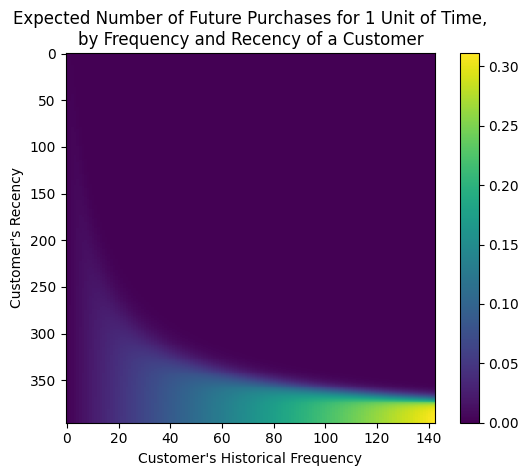
\includegraphics[width=0.85\textwidth]{images/matriz-f-r.png}
	\caption{Matriz de Frecuencia, Recencia y Compras Esperadas}
	\label{fig:frc}
\end{figure}

\vspace{-5.5mm}

	Se puede apreciar que si un cliente ha interactuado más de 120 veces, y su última interacción la realizó luego de 350 días de estar activo, entonces se puede considerar como uno de los mejores clientes (abajo a la derecha). Los clientes menos activos son los que se encuentran en la esquina superior derecha: compraron mucho rápido y no lo han vuelto a hacer en semanas.

	También está la “cola” alrededor de las coordenadas (20, 300). Eso representa al cliente que compra con poca frecuencia, pero que se ha visto recientemente, por lo que podría volver a comprar; no se tiene seguridad de si ha dejado de ser cliente o solo está en un periodo entre compras.
	
\subsubsection{Matriz de Frecuencia, Recencia y Probabilidad de vida}

Otra información interesante a evaluar es la relación entre la frecuencia, recencia y la probabilidad de vida de un cliente.

\begin{figure}[H]
	\centering 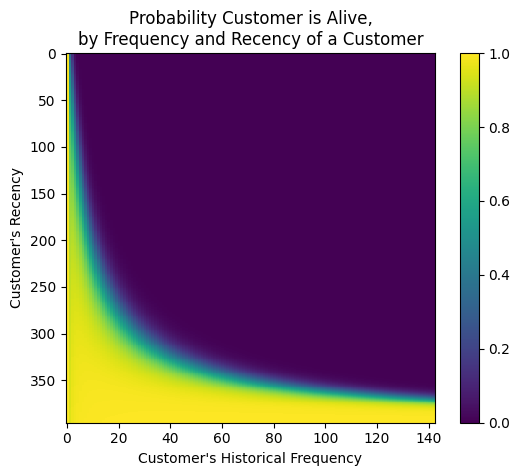
\includegraphics[width=0.80\textwidth]{images/probabilidad-vida.png}
	\caption{Matriz de Frecuencia, Recencia y Probabilidad de vida}
	\label{fig:frp}
\end{figure}

De forma similar a la matriz anterior, si los clientes tienen una frecuencia alta de compra y se han visto durante tiempos prolongados, su probabilidad de ser clientes es muy alta (abajo y a la derecha). De igual manera si un cliente se ha visto recientemente tiene una alta probabilidad de estar activo (arriba a la izquierda).

\subsubsection{Evaluación del ajuste del modelo}

En el siguiente gráfico se evalúan los parámetros de ajuste del modelo, para ello se comparan los datos que se utilizaron para ajustar el modelo con datos artificiales simulados con los parámetros del modelo ajustado.

\begin{figure}[H]
	\centering 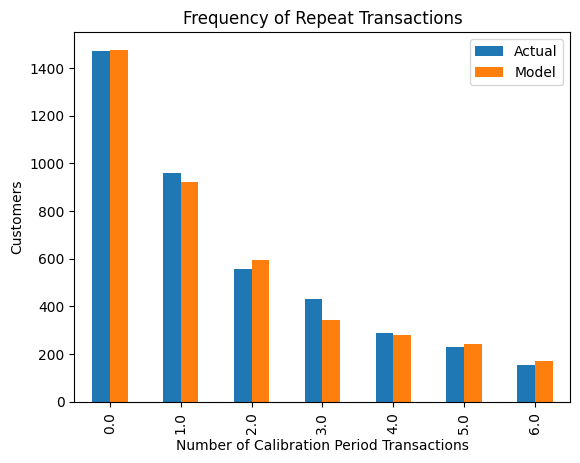
\includegraphics[width=0.80\textwidth]{images/ajuste-modelo.png}
	\caption{Comparación entre el modelo y datos generados}
	\label{fig:ajuste}
\end{figure}

Se puede observar que los datos reales y los datos simulados se alinean bien, esto prueba que el modelo es bueno y representa muy bien el comportamiento de los clientes.

\subsubsection{Validación Cruzada}

Se puede dividir el conjunto de datos en un grupo de datos de período de calibración y otro grupo de datos de reserva. Esto es importante ya que se quiere probar cómo funciona el modelo en datos que aún no se han visto. La biblioteca lifetimes contiene una función para particionar el conjunto de datos:

\begin{lstlisting}[language=Python, caption=Validación en modelo.ipynb]
summary_cal_holdout = calibration_and_holdout_data(transactional_data, 'CustomerNo', 'Date',                                            calibration_period_end='2019-06-09', observation_period_end='2019-12-09')
\end{lstlisting}

Luego de dividir la data, se procede a ajustar el modelo con los datos del periodo de calibración:

\begin{lstlisting}[language=Python, caption=Validación en modelo.ipynb]
model.fit(summary_cal_holdout['frequency_cal'], summary_cal_holdout['recency_cal'], summary_cal_holdout['T_cal'])
\end{lstlisting}

Finalmente, se compara las compras del periodo de reserva, con las compras esperadas por el modelo en ese mismo periodo:

\begin{figure}[H]
	\centering 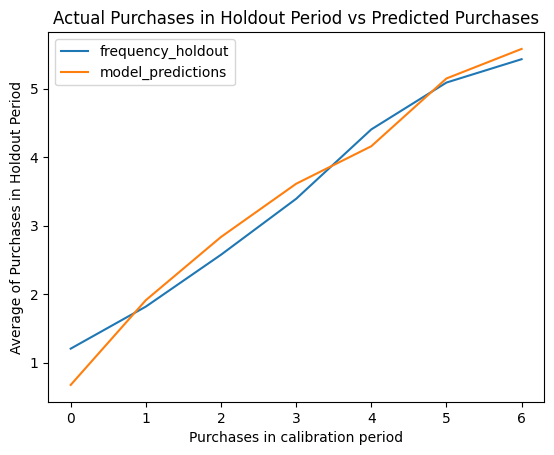
\includegraphics[width=0.80\textwidth]{images/comparacion.png}
	\caption{Comparación entre compras predecidas y compras reales}
	\label{fig:comp}
\end{figure}

Se puede apreciar una gran similitud entre las compras reales del periodo donde el modelo no tiene conocimiento y las compras que el modelo predijo, viendo esto y las pruebas anteriores podemos concluir que el modelo tiene un rendimiento suficientemente bueno para ser usado en el sistema.

\subsection{API}

Para verificar que la API cumple los requerimientos, se realizaron pruebas mediante un software para hacer peticiones HTTP llamado Insomnia, con el se realizaron varias llamadas al recurso /conditional-probability-alive con diferentes parámetros de entrada, esto con la finalidad de verificar que la respuesta cumple con los objetivos.

\begin{figure}[H]
	\centering 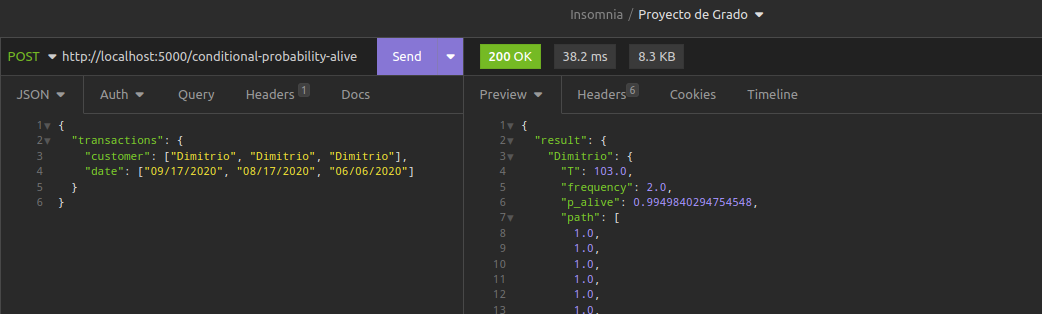
\includegraphics[width=0.80\textwidth]{images/3.png}
	\caption{Prueba con datos válidos}
	\label{fig:api1}
\end{figure}

En el primer caso se envió una petición válida con información sobre varias transacciones y el recurso responde correctamente a la solicitud.

\begin{figure}[H]
	\centering 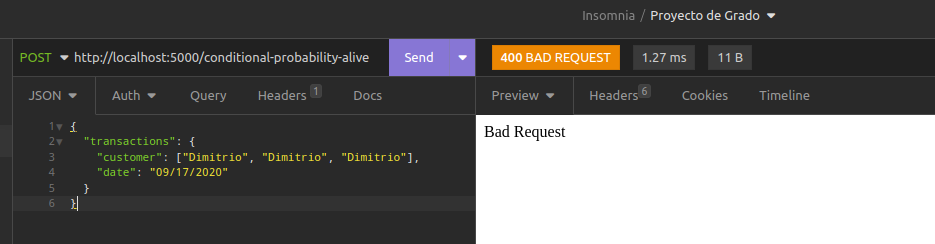
\includegraphics[width=0.80\textwidth]{images/4.png}
	\caption{Prueba con datos inválidos}
	\label{fig:api2}
\end{figure}

En el segundo caso se envió una petición inválida a la API y esta responde con el mensaje adecuado.

\subsection{Aplicación Web}

Ya que el listado de transacciones debe tener un formato especifico, se validó la entrada del usuario para garantizar esta estructura, para ello se muestra un texto de ayuda y mensajes con información sobre los diferentes errores de entrada posibles.

\begin{figure}[H]
	\centering 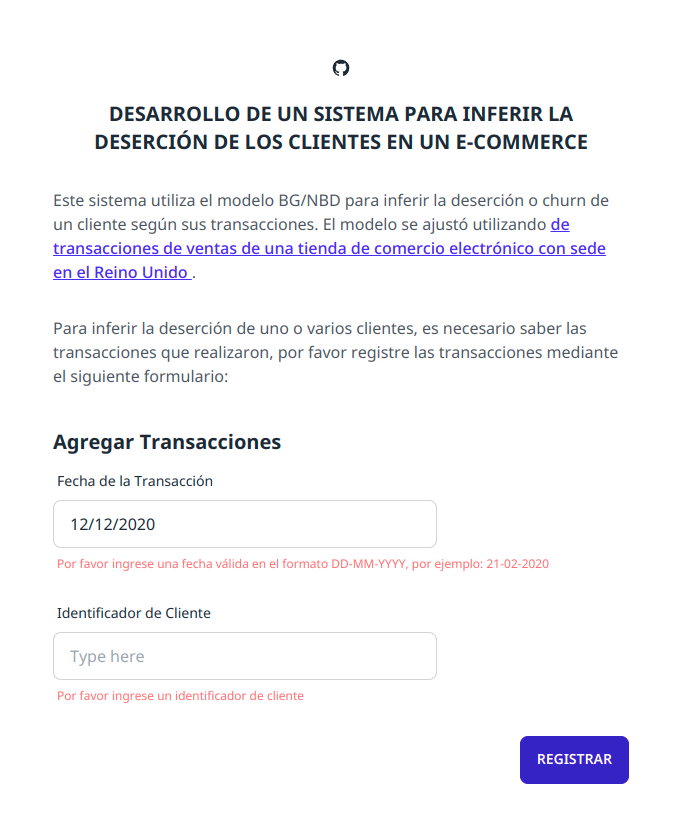
\includegraphics[width=0.80\textwidth]{images/6.png}
	\caption{Interfaz con errores de validación}
	\label{fig:ui1}
\end{figure}

\section{Resultados}

En esta sección se muestra el funcionamiento del modelo obtenido, las predicciones que arrojó según ciertos parámetros de ejemplo y la interpretación de estos resultados.

\subsection{Modelo}

A continuación se van a presentar ejemplos de clientes dentro del dataset, sus resultados y un análisis de la información obtenida:

\subsubsection{Ejemplo 1}

En este ejemplo se aprecia el comportamiento de un cliente que realizó dos compras consecutivas, al inicio la probabilidad de ser considerado un cliente baja con una mayor rapidez, luego de que el cliente realiza otra compra se puede ver que la probabilidad ahora disminuye más lentamente. Finalmente luego de la cuarta compra se puede observar que este cliente tiene una relación saludable con la tienda y tiene un patrón de compra definido.

\begin{figure}[H]
	\centering 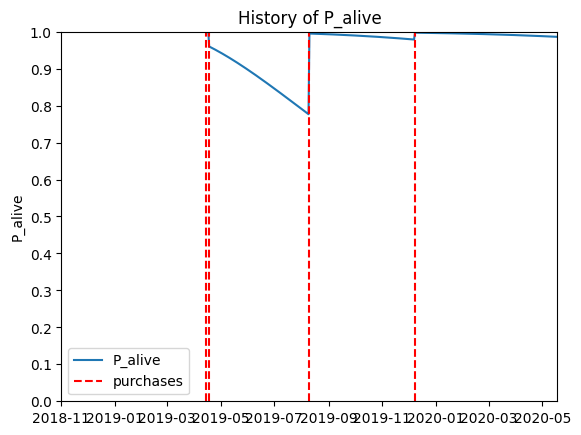
\includegraphics[width=0.60\textwidth]{images/e1.png}
	\caption{Probabilidad de vida Ejemplo 1}
	\label{fig:e1}
\end{figure}

\subsubsection{Ejemplo 3}

Este caso es de interés ya que se puede apreciar a un cliente que compra muy seguido durante todo el año, luego de pasar unos días sin comprar, el modelo penaliza fuertemente su probabilidad de seguir siendo cliente ya que no mantiene su comportamiento anterior.

\begin{figure}[H]
	\centering 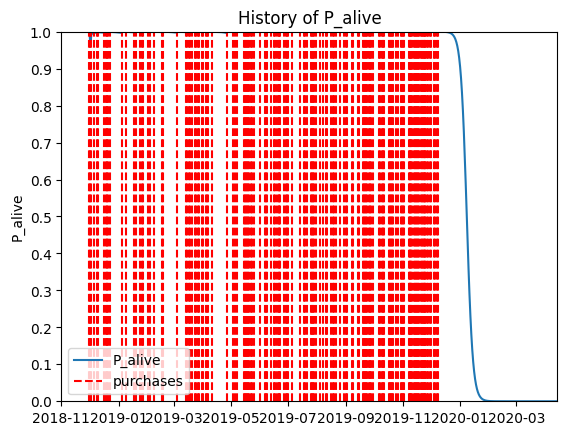
\includegraphics[width=0.60\textwidth]{images/e3.png}
	\caption{Probabilidad de vida Ejemplo 3}
	\label{fig:e3}
\end{figure}

\subsubsection{Ejemplo 4}

En este ejemplo el cliente realizó dos compras y durante el año la probabilidad de vida del cliente fue disminuyendo pero no fue descartado, como vemos luego el cliente regresó y se completó su patrón de compra.

\begin{figure}[H]
	\centering 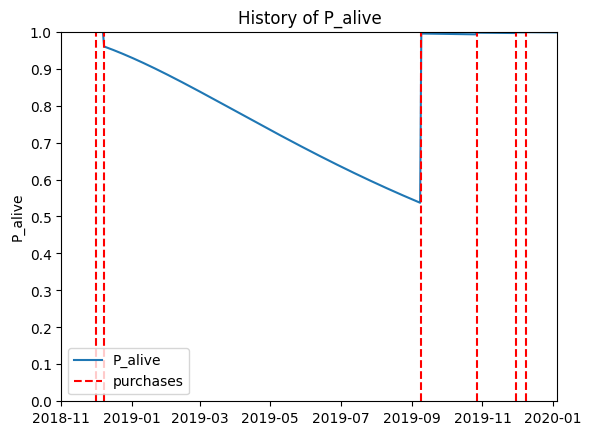
\includegraphics[width=0.60\textwidth]{images/e4.png}
	\caption{Probabilidad de vida Ejemplo 4}
	\label{fig:e4}
\end{figure}

\subsection{API y Aplicación Web}

A continuación se puede observar los resultados obtenidos al utilizar el sistema para predecir la probabilidad de deserción de un cliente dada una lista de transacciones del mismo.

	Esta prueba verifica que la integración entre la aplicación web y la API funciona correctamente y que el sistema está cumpliendo con la funcionalidad esperada.
	
\begin{figure}[H]
	\centering 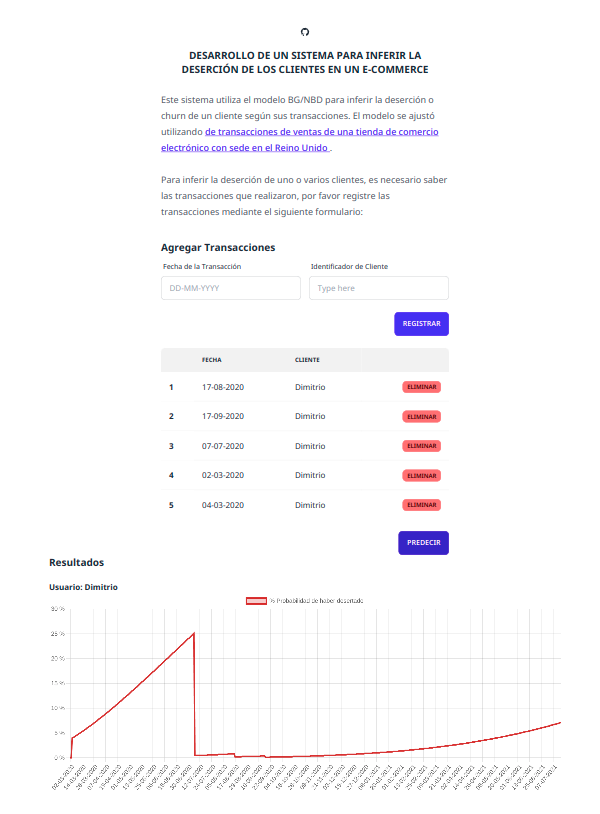
\includegraphics[width=0.60\textwidth]{images/7.png}
	\caption{Interfaz con resultados}
	\label{fig:ui2}
\end{figure}
